\documentclass[conference,a4paper]{IEEEtran}
\IEEEoverridecommandlockouts
\usepackage{cite}
\usepackage{amsmath,amssymb}
\usepackage{graphicx}
\usepackage[utf8]{inputenc}
\usepackage{url}
\makeatletter
\newcommand{\linebreakand}{\end{@IEEEauthorhalign}\hfill\mbox{}\par\mbox{}\hfill\begin{@IEEEauthorhalign}}
\makeatother
\begin{document}

\title{Detection and Classification of Exoplanet Transit Signals in Kepler and TESS Light Curves Using Signal Processing and Machine Learning}

\author{\IEEEauthorblockN{\makebox[\textwidth][c]{\parbox[t]{0.32\textwidth}{\centering Girinath A\\[3pt]
\footnotesize Register No: URK23EC4018\\
\textit{Dept. of Electronics and Communication Engg.}\\
\textit{Karunya Institute of Technology and Sciences}\\
Coimbatore, Tamil Nadu, India\\
girinatha@karunya.edu.in}\hspace{0.02\textwidth}\parbox[t]{0.32\textwidth}{\centering Akilan S\\[3pt]
\footnotesize Register No: URK23EC1001\\
\textit{Dept. of Electronics and Communication Engg.}\\
\textit{Karunya Institute of Technology and Sciences}\\
Coimbatore, Tamil Nadu, India\\
akilans@karunya.edu.in}\hspace{0.02\textwidth}\parbox[t]{0.32\textwidth}{\centering Misham Samuel Daystar\\[3pt]
\footnotesize Register No: URK23EC4004\\
\textit{Dept. of Electronics and Communication Engg.}\\
\textit{Karunya Institute of Technology and Sciences}\\
Coimbatore, Tamil Nadu, India\\
mishamsamueldaystar@karunya.edu.in}}\\[10pt]
\makebox[\textwidth][c]{\parbox[t]{0.32\textwidth}{\centering Sachin Sarlin K R S\\[3pt]
\footnotesize Register No: URK23EC4009\\
\textit{Dept. of Electronics and Communication Engg.}\\
\textit{Karunya Institute of Technology and Sciences}\\
Coimbatore, Tamil Nadu, India\\
sachinsarlin@karunya.edu.in}\hspace{0.04\textwidth}\parbox[t]{0.32\textwidth}{\centering Mrs. R. A. Rakhi\\[3pt]
\footnotesize Assistant Professor / Faculty Project Guide\\
\textit{Dept. of Electronics and Communication Engg.}\\
\textit{Karunya Institute of Technology and Sciences}\\
Coimbatore, Tamil Nadu, India\\
rakhira@karunya.edu.in}}}}

\maketitle

\begin{abstract}
Space telescopes such as Kepler and TESS find far more periodic dips in star brightness than people can check by hand, and most of these dips are not planets. In this project we built TransitVet, an open pipeline that takes the light curve of a star, searches it for repeating dips, and gives each signal a calibrated score and a three-way call: keep, drop, or needs a person. We first reproduced the AstroNet convolutional network on Kepler DR24 (accuracy 0.955, ROC-AUC 0.989) and showed that splitting the data by star gives lower, more realistic numbers. Under one strict protocol (split by star, every choice made on validation stars, test stars used once) we compared a threshold rule, gradient boosting, AstroNet, a pretrained Transformer and a Mamba-2 state-space model. The released tool combines gradient boosting, Mamba-2 and the Transformer. On held-out stars it reaches a precision-recall AUC of 0.963 on Kepler (2,373 signals) and 0.950 on TESS (1,000 signals), within the uncertainty of the published ExoMiner++ scores on shared signals. A class-conditional conformal check keeps at least 95\% coverage for both classes. An injection-recovery test with 90 synthetic planets shows that the search finds half of them at a signal-to-noise ratio of about 10. We release the code, a web dashboard and scores for 4,408 open TESS signals.
\end{abstract}

\begin{IEEEkeywords}
Exoplanets, Transit photometry, Kepler, TESS, Deep learning, Gradient boosting, Mamba-2, Transformer, Conformal prediction, Signal processing
\end{IEEEkeywords}

\section{Introduction}
A planet that passes in front of its star blocks a small part of the starlight. The star's brightness, recorded over time as a light curve, then shows a small dip that repeats once every orbit. The Kepler \cite{r1} and TESS \cite{r2} space telescopes have measured light curves for hundreds of thousands of stars and found tens of thousands of such periodic signals. Only a minority are planets. The rest are eclipsing binary stars, light from a nearby eclipsing star that falls on the same pixels, star spots and pulsation, or instrument noise. Deciding which signals deserve telescope time is called vetting. Done by hand it is slow, and experts do not always agree.

From a signal-processing point of view, vetting is a detection and classification problem on a noisy, gappy time series. The signal of interest is a short, shallow, periodic dip; the noise includes slow trends, correlated noise and other periodic signals. Machine learning has become a standard aid. AstroNet \cite{r3} showed that a one-dimensional convolutional network on phase-folded light curves separates Kepler planet candidates from false positives well. Two practical questions still get less attention in the papers we read. First, how much do the reported numbers depend on how the data are split? Second, how should a tool show its uncertainty, when a confident wrong answer wastes telescope time?

To answer these questions, this project makes the following contributions:

\begin{itemize}
\item We reproduce AstroNet on Kepler DR24 with its original split by signal and with a stricter split by star.
\item We compare five models (a rule, gradient boosting, AstroNet, a pretrained Transformer and Mamba-2) on Kepler and TESS under one protocol.
\item We add a class-conditional conformal check that sends signals the models cannot place to a person instead of guessing.
\item We test the whole pipeline with synthetic planets, measuring both what the search finds and what the classifier then calls it.
\item We release an open web dashboard and scores for 4,408 TESS signals that are still open.
\end{itemize}
All positive outputs are planet candidates; we make no claim of planet discoveries.

\section{Related Work}
Shallue and Vanderburg \cite{r3} introduced the global view (whole orbit) and local view (around the dip) and trained a convolutional network on the Kepler DR24 training set, reaching an accuracy of 0.960. The idea was moved to TESS by Yu et al. \cite{r4}, and Tey et al. \cite{r5} improved it for TESS full-frame images, reporting a precision-recall AUC of 0.965. These models see only the light curve. ExoMiner \cite{r6} added the diagnostics a human vetter uses (odd and even transits, secondary eclipses, centroid motion) and was used to validate 301 Kepler planets. ExoMiner++ \cite{r7} extends this to TESS 2-minute data and publishes scores for all TESS signals; it is our main external comparison.

Transformers have also been applied to vetting \cite{r8}. Mamba-2 \cite{r9} is a newer state-space model whose cost grows only linearly with sequence length. In the vetting papers we read, we did not find it applied to folded light curves. Conformal prediction \cite{r10}, \cite{r11} gives prediction sets with a coverage guarantee that does not depend on the model. ExoVeil \cite{r12} used it to rank transit detections; we use its class-conditional form to give a separate guarantee for planets and for false signals. Most vetting papers report classifier metrics on catalogue signals only. We also run injections through the full pipeline, because a planet that is found but then called a false alarm is still lost to the user.

\section{System Methodology and Workflow}
Fig. 1 shows the complete pipeline. A user gives a Kepler (KIC) or TESS (TIC) star number. The pipeline downloads the light curve, cleans and detrends it, searches it for periodic dips, and builds two folded views and a set of vetting statistics for each signal. Three models score each signal, a logistic combiner merges their scores, and a verdict and a 95\% check are given. The same code runs in the web dashboard and in a batch mode for many stars.

\begin{figure*}[!t]
\centering
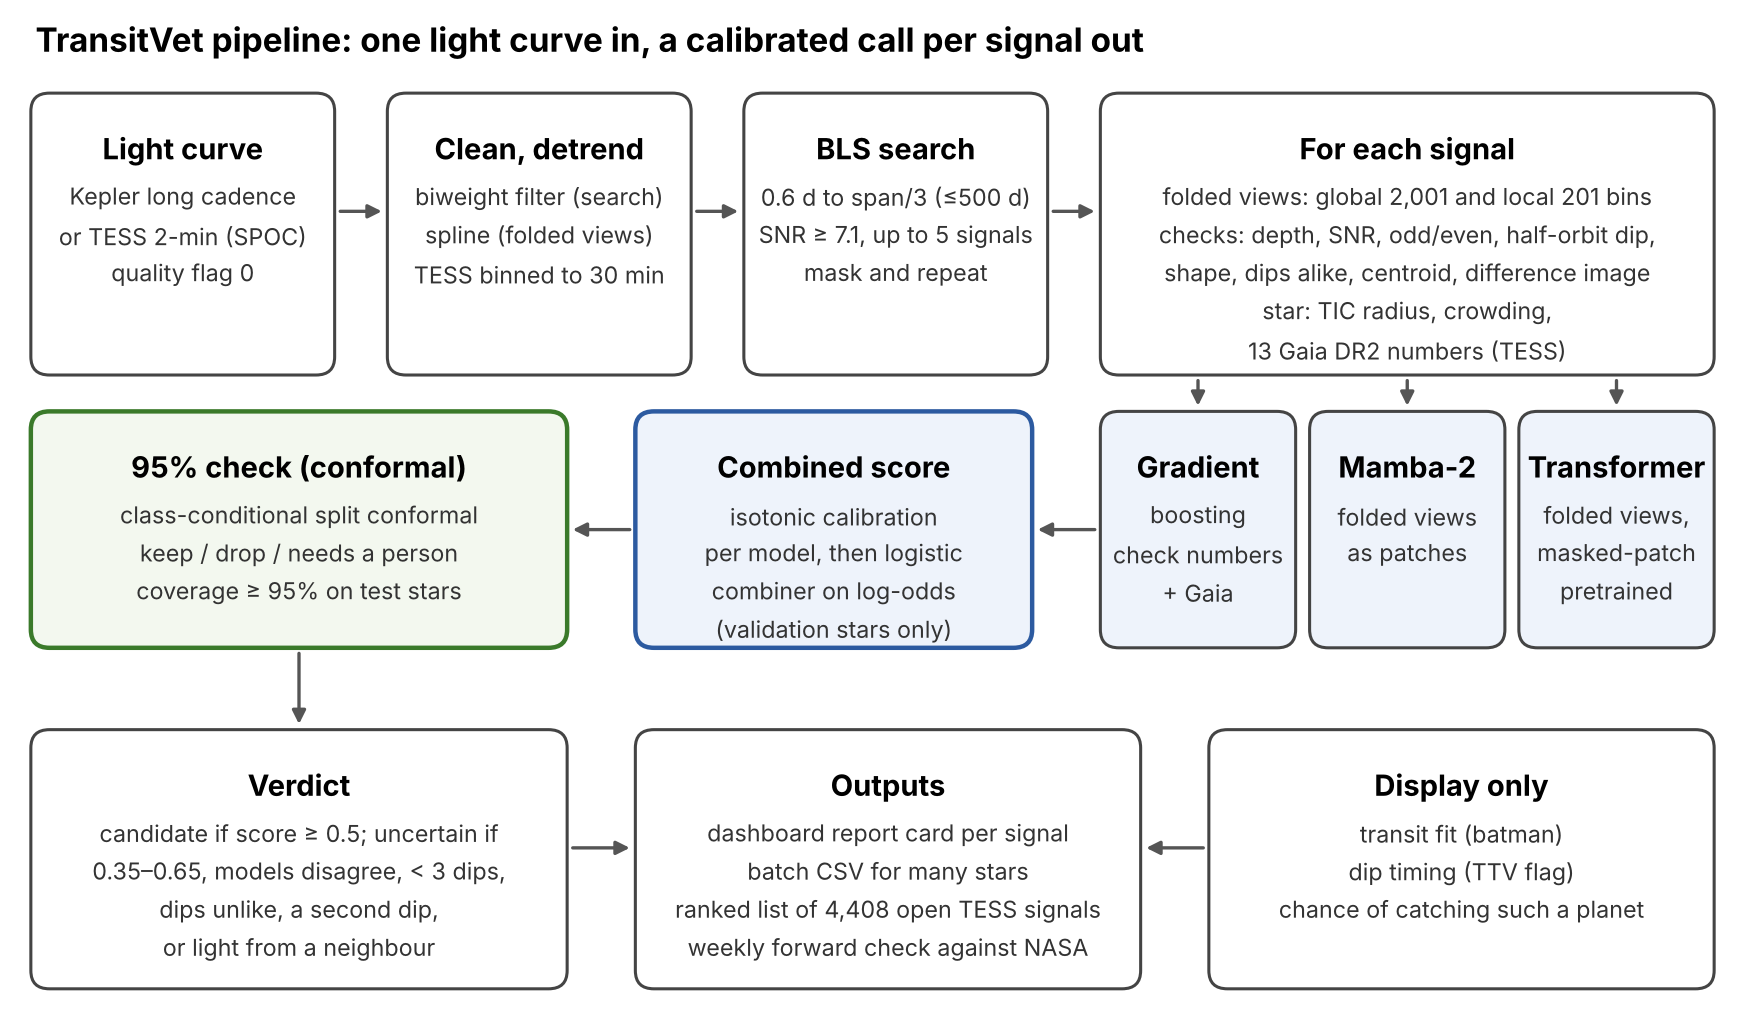
\includegraphics[width=0.8\textwidth]{figures/fig_pipeline.png}
\caption{Complete TransitVet pipeline. The three models feed a logistic combiner. The combined score sets the verdict, and a separate conformal combiner sets the 95\% check. The transit fit, dip-timing check and detection chance are display only.}
\label{fig:pipeline}
\end{figure*}
\subsection{Cleaning and Detrending}
We keep only points with quality flag 0. TESS data are binned to 30 minutes so that Kepler and TESS views have similar sampling. For the search, slow brightness trends are removed with a time-windowed biweight filter (w\={o}tan \cite{r13}) with a 1-day window, which acts as a robust low-pass filter. Upward outliers above 5 robust standard deviations are removed; dips are kept.

\subsection{Transit Search}
Repeating dips are found with the box least squares (BLS) method \cite{r14}, which fits a box-shaped dip at every trial period from 0.6 days to a third of the data span. A signal must reach a BLS signal-to-noise ratio of at least 7.1. Up to five signals are kept per star, and each is masked before the next search.

\subsection{Folded Views and Vetting Statistics}
Each signal is folded at its period. As in AstroNet \cite{r3}, a global view of 2,001 bins covers the whole orbit and a local view of 201 bins covers $\pm$4 transit durations (Fig. 2). From the detrended curve we also compute ten statistics that a human vetter would check: depth and signal-to-noise, odd/even depth difference, a dip at half an orbit (secondary eclipse), a U-versus-V shape ratio, number of dips, period, duration and coverage.

\begin{figure}[!ht]
\centering
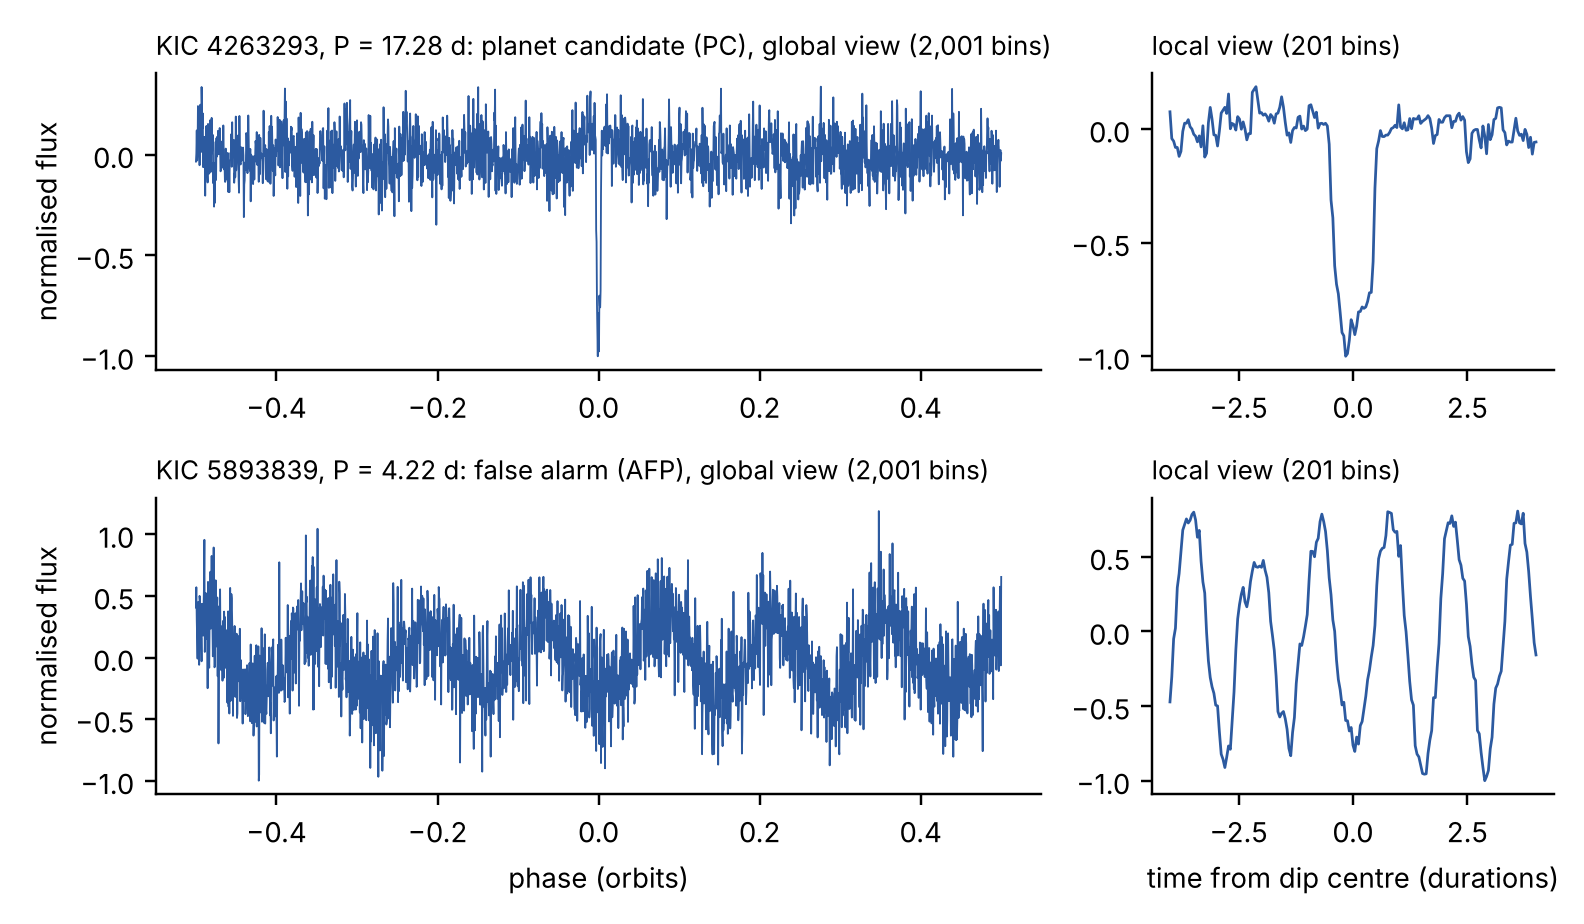
\includegraphics[width=\columnwidth]{figures/fig_views.png}
\caption{Global and local views of two Kepler test signals: a planet candidate (top) and a false alarm on a variable star (bottom).}
\label{fig:views}
\end{figure}
\subsection{Star and Pixel Context}
For context we add the star radius and the contamination ratio from the TESS Input Catalog, an estimated planet size, and the shift of the light centre during the dip. For TESS stars we also query Gaia DR2 \cite{r15} and add 13 numbers about the star and its neighbours, such as how many sources lie within one and two TESS pixels and how deep a dip the brightest neighbour would need to fake the signal. A difference-image check fits the out-of-dip minus in-dip image to find where the dip comes from; it is used as a rule, not as a score input.

\section{Dataset Description}
Table I lists the data. For Kepler we use the Q1--Q17 DR24 signals and labels \cite{r16}: planet candidate = 1; astrophysical false positive and non-transiting phenomenon = 0. For TESS we use the TESS Objects of Interest table \cite{r17} from the NASA Exoplanet Archive (downloaded 1 November 2026) with 2-minute light curves: confirmed and known planets = 1; false positives and false alarms = 0. Signals still marked as candidates have no final label; we use them only for pretraining and score them separately.

All splits are by star: every signal of a star goes to the same part. Signals on one star share noise and often the same cause (for example, both eclipses of a binary), so a split by signal lets a model learn the star instead of the signal. All 6,910 TESS objects with 2-minute data were processed with no failures.

\begin{table}[!ht]
\caption{Data Sets and Split by Star}
\centering\footnotesize\setlength{\tabcolsep}{4pt}
\begin{tabular}{lccl}
\hline
\textbf{Set} & \textbf{Signals} & \textbf{Stars} & \textbf{Split (train / val / test)} \\
\hline
Kepler DR24 & 15,737 & 9,865 & 11,053 / 2,311 / 2,373 \\
TESS labelled & 2,502 & 2,357 & 1,243 / 259 / 1,000 \\
TESS open (unlabelled) & 4,408 & 4,294 & scored only \\
\hline
\end{tabular}
\end{table}
The Kepler test set holds 519 planet candidates and 1,854 false signals on 1,480 stars. The TESS test set holds 542 planets and 458 false signals on 943 stars. TESS uses a 40\% test share so that its results have usable error bars.

\section{Model Architectures}
\subsection{Compared Models}
Table II summarises the models. All settings were chosen on validation stars only.

\begin{table*}[!t]
\caption{Models Compared}
\centering\footnotesize\setlength{\tabcolsep}{4pt}
\begin{tabular}{lll}
\hline
\textbf{Model} & \textbf{Input} & \textbf{Main settings} \\
\hline
Threshold rule & depth, SNR, odd/even & 3 limits by grid search \\
Gradient boosting (GB) & statistics + context (+ Gaia on TESS) & histogram GB, up to 500 iterations, 5 seeds \\
AstroNet CNN & both views & as in \cite{r3}, 9.9 M parameters \\
Patch Transformer & 89 patches of the views & 4 layers, width 128, 0.55 M parameters, masked pretraining \\
Mamba-2 & same 89 patches & 4 bidirectional blocks, width 64, state 32 \\
\hline
\end{tabular}
\end{table*}
The Transformer cuts the two views into 63 global and 26 local patches. It is first pretrained without labels by hiding 40\% of the patches and learning to rebuild them, using 15,456 views from Kepler training signals and open TESS signals. Mamba-2 was written in plain PyTorch in its matrix form; it matches the step-by-step recurrence to 1.5$\times10^{-8}$. Because a folded light curve has no arrow of time, each block runs in both directions. For TESS, the neural models are trained on Kepler and then fine-tuned on TESS training stars.

\subsection{Combined Score and Verdict}
Each model's output is calibrated with isotonic regression on validation stars, so that a score of 0.8 means about 8 in 10 such signals are planets. A logistic regression on the three calibrated log-odds (GB, Mamba-2, Transformer) gives the combined score. The verdict is candidate if the score is at least 0.5 and false alarm otherwise. It becomes uncertain if the score is between 0.35 and 0.65, all three models disagree with it, fewer than 3 dips are seen, a second dip appears at the same period, the difference image points to a neighbour, or the single dips do not look alike.

\subsection{The 95\% Check}
We split the validation stars into two halves. Half A fits a second combiner and half B (1,157 Kepler and 129 TESS signals) calibrates it. With class-conditional split conformal prediction at $\alpha$ = 0.05 we set one cut-off per class. For a new signal, ``planet'' stays in the prediction set if its score passes the planet cut-off, and likewise for ``false alarm''. If only planet remains the call is keep; if only false alarm remains it is drop; otherwise the signal goes to a person. If new signals behave like the calibration signals, at least 95\% of real planets keep ``planet'' in their set and at least 95\% of false signals keep ``false alarm''. The tool also sends a signal to a person when this call and the combined score disagree.

\subsection{Evaluation Metric}
The main metric is the area under the precision-recall curve (PR-AUC), which is more informative than ROC-AUC when classes are unbalanced. Uncertainties come from 2,000 bootstrap resamples of test stars. Test stars were scored once, at the end.

\section{Experimental Results and Performance Evaluation}
\subsection{Reproducing AstroNet}
Under AstroNet's own split by signal (test 1,574 signals), the average of our 10 PyTorch models reaches accuracy 0.955 and ROC-AUC 0.989, against 0.960 and 0.988 in the original paper \cite{r3}. Under a split by star with the same proportions, the same setup gives accuracy 0.951, ROC-AUC 0.982 and PR-AUC 0.943 (0.948 under the split by signal). The two test sets differ, so this is not a paired comparison, but the drop is in the direction expected if a split by signal leaks information through shared stars.

\subsection{Kepler Results}
Table III gives the Kepler test results. Light-curve-only gradient boosting reaches 0.885. Adding star and pixel context lifts it to 0.947. The AstroNet CNN is the best single neural model (0.941). The combined score reaches 0.963 (95\% interval 0.945--0.980). At the 0.5 rule it rejects 1,804 of 1,854 false signals and keeps 482 of 519 planet candidates. Fig. 3 shows the precision-recall curves.

\begin{table*}[!t]
\caption{Kepler Test PR-AUC (2,373 Signals, Split by Star)}
\centering\footnotesize\setlength{\tabcolsep}{4pt}
\begin{tabular}{lcc}
\hline
\textbf{Model} & \textbf{PR-AUC (mean $\pm$ s.d.)} & \textbf{5-model average} \\
\hline
Threshold rule & 0.463 & -- \\
GB, light-curve statistics only & 0.885 $\pm$ 0.005 & -- \\
Transformer, no pretraining & 0.923 $\pm$ 0.002 & 0.930 \\
Mamba-2 & 0.926 $\pm$ 0.004 & 0.934 \\
Transformer, pretrained & 0.931 $\pm$ 0.002 & 0.932 \\
AstroNet CNN & 0.941 $\pm$ 0.003 & 0.947 \\
GB with star and pixel context & -- & 0.947 \\
\textbf{Combined (GB + Mamba-2 + Transformer)} & -- & \textbf{0.963} \\
\hline
\end{tabular}
\end{table*}
\begin{figure}[!ht]
\centering
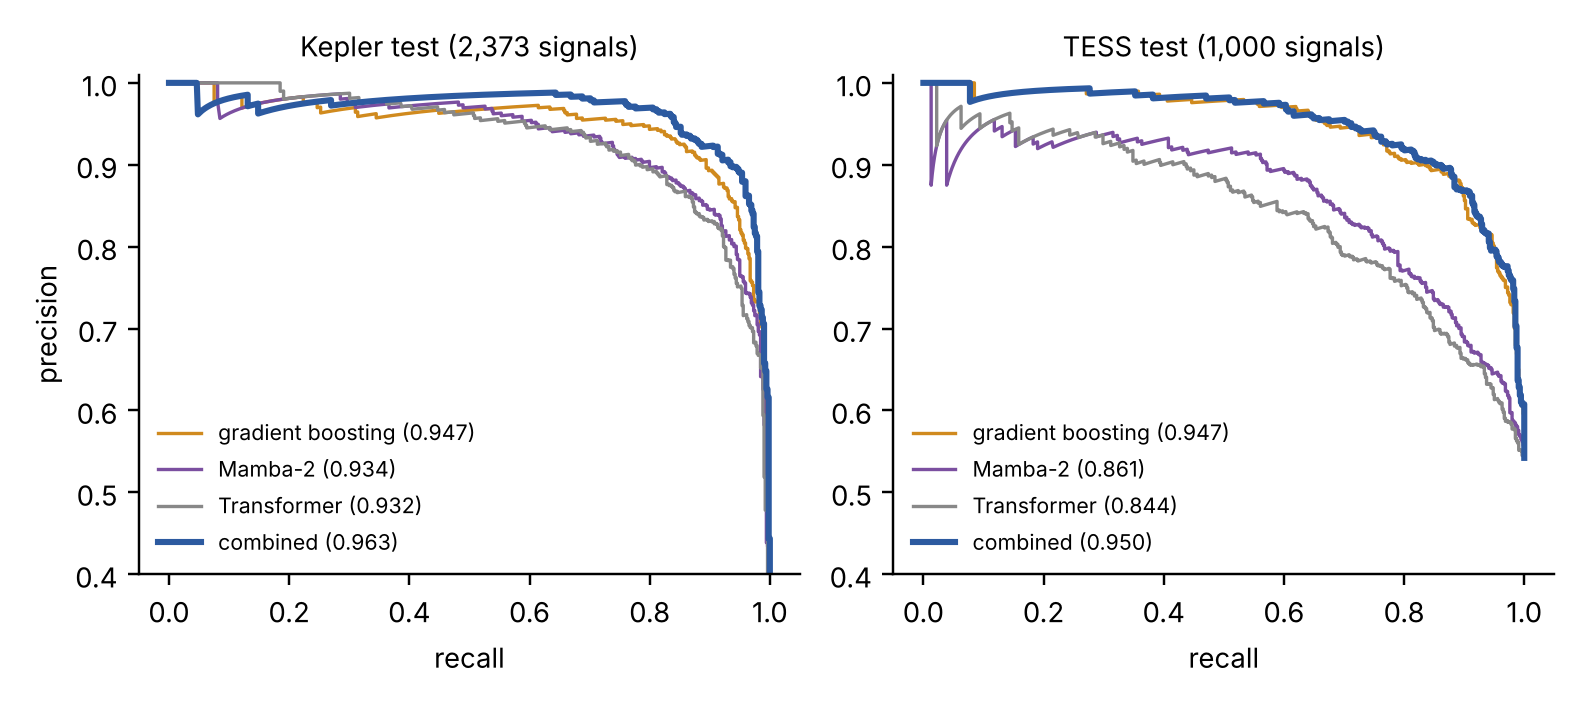
\includegraphics[width=\columnwidth]{figures/fig_pr_curves.png}
\caption{Precision-recall curves on test stars for the three models in the tool and their combination (PR-AUC in brackets). Left: Kepler. Right: TESS.}
\label{fig:pr_curves}
\end{figure}
Replacing Mamba-2 with the CNN in the combiner gives 0.968; the difference is within the bootstrap uncertainty, so we keep the smaller Mamba-2 model. Masked pretraining helps the Transformer most when labels are scarce: with 10\% of the labels it gains 0.026 PR-AUC. At every label fraction the CNN stays ahead, so at this data size neither attention nor a state-space model beats the convolutional baseline on Kepler views.

\subsection{TESS Results and Transfer from Kepler}
Table IV shows that for the neural models, training on Kepler and fine-tuning on TESS beats training on TESS alone, as expected with only 1,243 TESS training signals. Models used unchanged from Kepler are poorly calibrated on TESS (calibration error 0.146 for the CNN); isotonic calibration on TESS validation stars brings this to 0.058.

\begin{table}[!ht]
\caption{TESS Test PR-AUC (1,000 Signals; Random = 0.542)}
\centering\footnotesize\setlength{\tabcolsep}{4pt}
\begin{tabular}{lccc}
\hline
\textbf{Model} & \textbf{Kepler, unchanged} & \textbf{Fine-tuned} & \textbf{TESS only} \\
\hline
GB, light-curve statistics & 0.800 & -- & 0.876 \\
AstroNet CNN & 0.835 & 0.858 & 0.822 \\
Transformer, pretrained & 0.819 & 0.842 & 0.795 \\
Mamba-2 & 0.840 & 0.852 & 0.808 \\
\hline
\end{tabular}
\end{table}
On TESS, star context does most of the work: planet size and contamination alone lift GB from 0.883 to 0.940, and the 13 Gaia numbers lift it to 0.947. The combined score reaches 0.950 (95\% interval 0.933--0.964). With Gaia, false signals rejected at the 0.5 rule rise from 363 to 382 of 458, while planets kept go from 492 to 493 of 542. The difference-image check flags 113 of 458 false signals but only 19 of 542 planets; used as a rule, it moves 19 of the 76 false signals called candidates to uncertain, at the cost of 16 of 493 planet candidates.

\subsection{The 95\% Check}
Table V shows the check on test stars. Coverage meets the 95\% target for both classes on both missions. On Kepler the classes are well separated, so almost every signal gets a firm call: 90.6\% of keep calls are planet candidates and 98.9\% of drop calls are false. On TESS about a third of the signals go to a person, because the classes overlap more and the cut-offs rest on only 129 calibration signals; 95.6\% of TESS keep calls are planets. This is the intended behaviour: the tool says when it cannot separate a signal rather than giving a confident answer it cannot back up (Fig. 4).

\begin{table}[!ht]
\caption{95\% Check on Test Stars ($\alpha$ = 0.05)}
\centering\footnotesize\setlength{\tabcolsep}{4pt}
\begin{tabular}{lccccc}
\hline
\textbf{Mission} & \textbf{Planet cov.} & \textbf{False cov.} & \textbf{Keep} & \textbf{Drop} & \textbf{Person} \\
\hline
Kepler & 95.8\% & 95.3\% & 532 & 1,786 & 55 \\
TESS & 98.0\% & 96.3\% & 387 & 295 & 318 \\
\hline
\end{tabular}
\end{table}
\begin{figure*}[!t]
\centering
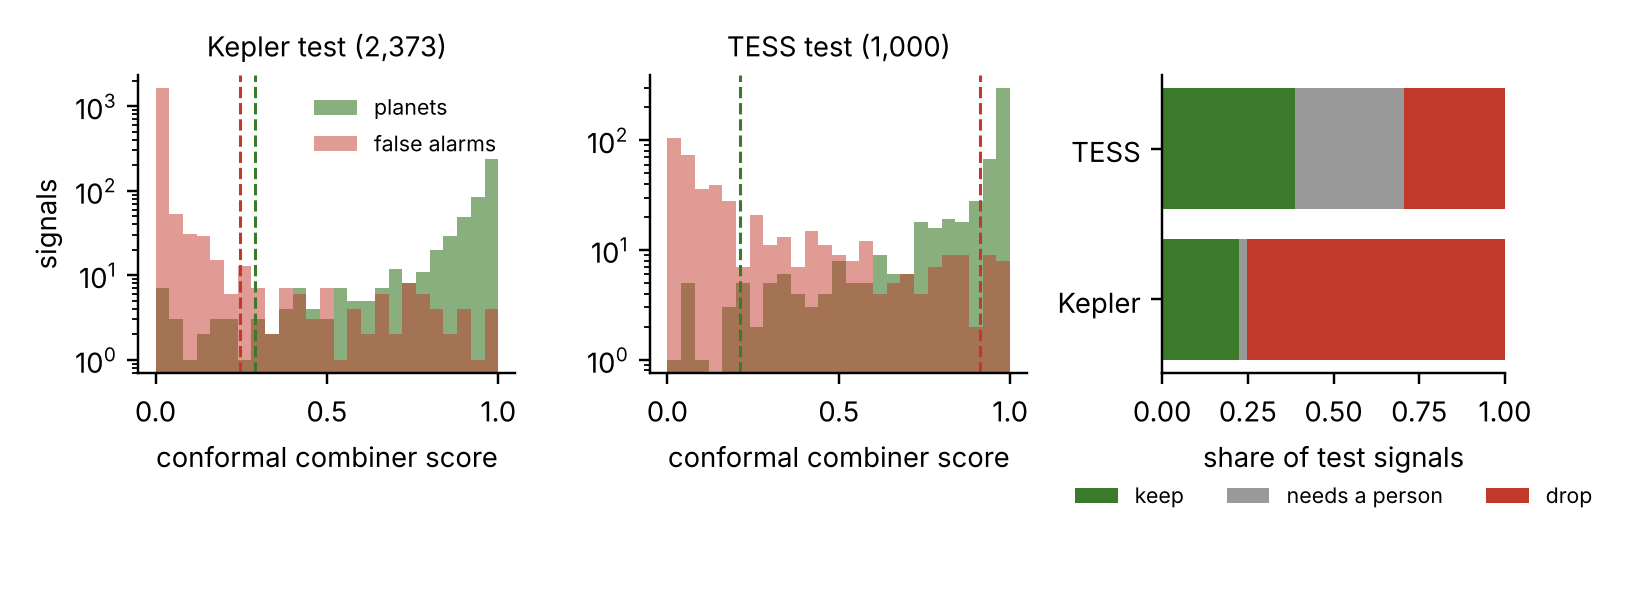
\includegraphics[width=0.95\textwidth]{figures/fig_conformal.png}
\caption{Left and centre: conformal-combiner scores of test planets and false signals with the two cut-offs (dashed). Right: share of test signals called keep, needs a person, or drop.}
\label{fig:conformal}
\end{figure*}
\subsection{Comparison with ExoMiner++}
ExoMiner++ \cite{r7} publishes scores for TESS 2-minute signals. We matched 542 of our 1,000 TESS test signals (347 planets, 195 false signals) by star and period. On these, TransitVet reaches a PR-AUC of 0.968 and ExoMiner++ 0.973; the difference of $-$0.005 has a bootstrap interval of $-$0.019 to +0.010, so the two are within the uncertainty. The comparison is not like for like: ExoMiner++ uses the mission's own pixel-level products, while TransitVet starts from light-curve files and catalogues and also scores its own detections.

\subsection{Injection-Recovery Test}
To measure what the whole pipeline can find, we added synthetic planets to the raw light curves of held-out test stars, using a batman transit model \cite{r18}, and ran everything unchanged. After leaving out planets with fewer than 3 dips in the data and planets on one giant star, 90 synthetic planets on 18 stars remained. Table VI and Fig. 5 show the result: the search finds half of the planets at an expected signal-to-noise ratio of about 10 and 90\% at about 16, and above 15 it found 36 of 37.

\begin{table}[!ht]
\caption{Injection-Recovery Result}
\centering\footnotesize\setlength{\tabcolsep}{4pt}
\begin{tabular}{lccc}
\hline
\textbf{Expected SNR} & \textbf{Planets} & \textbf{Recovered} & \textbf{Called candidate} \\
\hline
below 7.1 & 37 & 2 & 0 \\
7.1--15 & 16 & 9 & 2 \\
15--50 & 23 & 22 & 10 \\
50 and above & 14 & 14 & 4 \\
\hline
\end{tabular}
\end{table}
\begin{figure*}[!t]
\centering
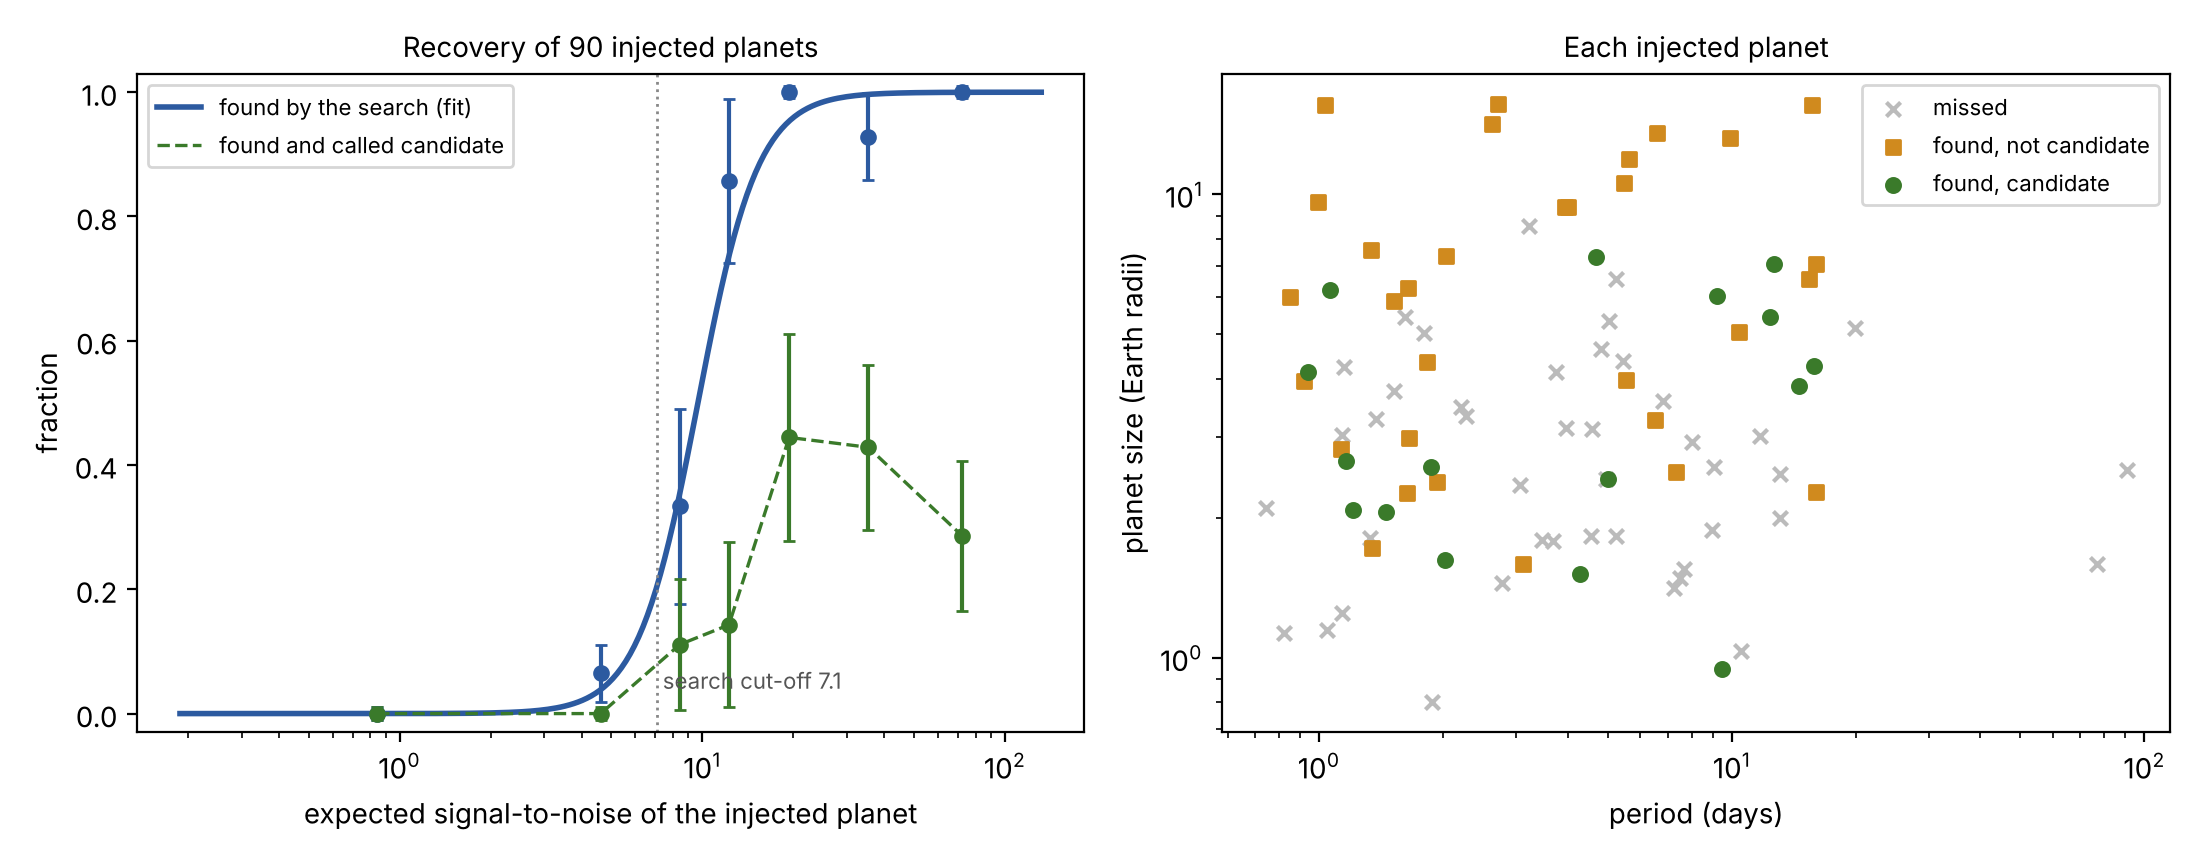
\includegraphics[width=0.95\textwidth]{figures/fig_sensitivity.png}
\caption{Left: share of synthetic planets recovered by the search (blue, logistic fit) and recovered and called candidate (green) against expected signal-to-noise ratio. Right: each synthetic planet by period and size.}
\label{fig:sensitivity}
\end{figure*}
The call on a recovered planet depends strongly on the host star. On 7 stars whose own signal is a known planet, 13 of 20 recovered planets were called candidates. On 10 stars whose own signal is a false positive, only 3 of 27 were. All three models scored these low, so the Gaia inputs alone are not the cause; the cause is not yet known [CHECK]. The dashboard therefore warns users to read a false-alarm call on such a star with care, and shows each star's chance of catching planets of 1, 2 and 4 Earth radii.

\subsection{Open TESS Signals and the Web Tool}
We scored all 4,408 TESS signals that were still open on 1 November 2026 (Fig. 6). The verdicts are 2,013 candidates, 792 uncertain and 1,603 false alarms. 1,304 are strong candidates (score at least 0.5, at least 3 dips, check says keep), and 398 of these have an estimated size under 4 Earth radii. On the 2,502 signals that ExoMiner++ also scores, the two place 72\% on the same side of 0.5. We froze these calls on 17 November 2026, and a weekly script compares them with new NASA dispositions as a forward test.

\begin{figure}[!ht]
\centering
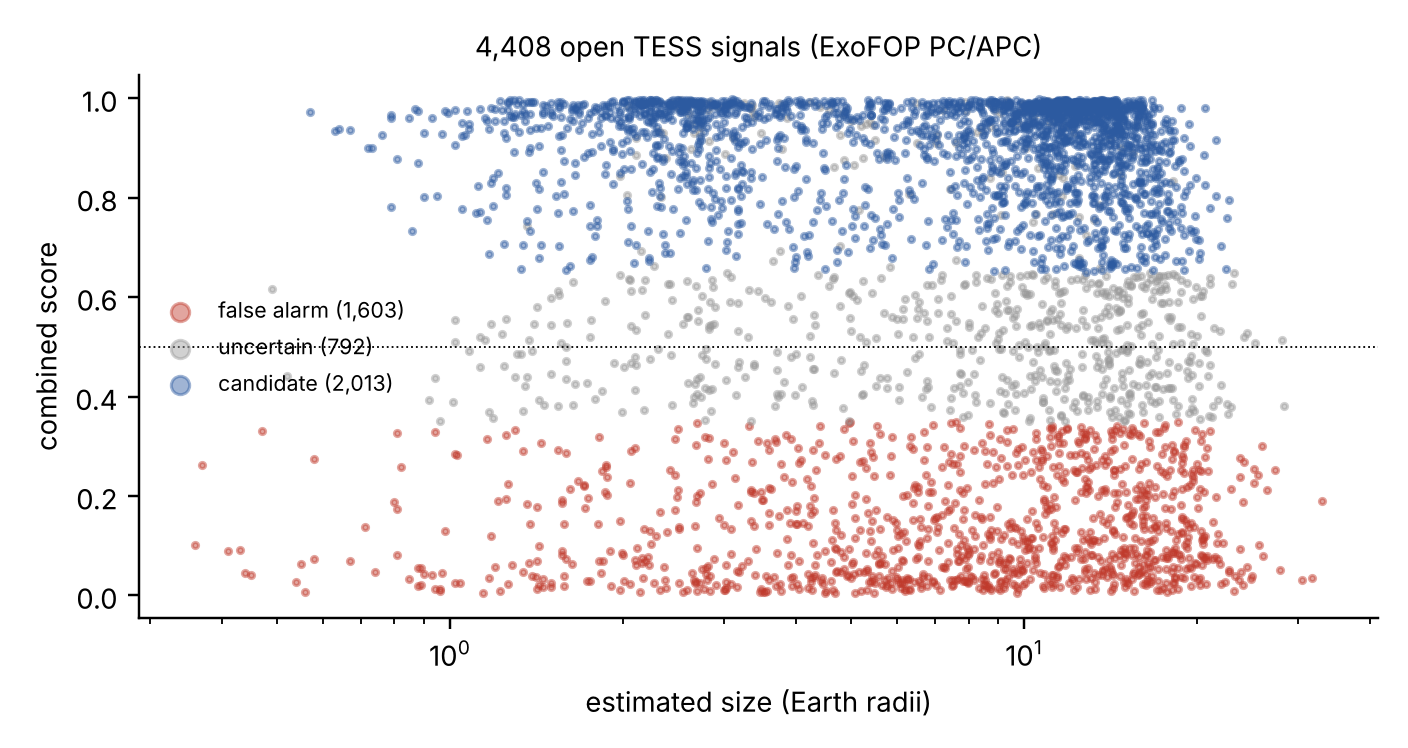
\includegraphics[width=\columnwidth]{figures/fig_open_signals.png}
\caption{Combined score against estimated planet size for the open TESS signals, coloured by verdict (636 signals without a size estimate not shown).}
\label{fig:open_signals}
\end{figure}
The Streamlit dashboard takes a star number and runs the full pipeline with a step-by-step view. It gives a plain-language summary and a report card for each signal, plays each dip as sound for accessibility, and shows the detection chance, upcoming dips and the ExoMiner++ score where one exists. Per signal, inference takes 7 $\mu$s for GB and 0.68 ms for the Transformer on a CPU; a whole star takes a few minutes, mostly for download, detrending and search.

\section{Discussion}
The results show that a light, open pipeline can reach PR-AUC values close to a large published system when star context is added, and that a split by star gives more realistic numbers than a split by signal. On TESS, gradient boosting with star context does most of the work; the TESS combiner gives Mamba-2 a weight of only 0.01. Newer architectures (Transformer, Mamba-2) did not beat the CNN at this data size; we ship Mamba-2 for its small size and equal combined performance, not because it is better on its own.

The work has limits. The official labels were made partly with the same evidence our context inputs use (centroid shifts, difference images, planet size), so part of the gain measures agreement with official vetting rather than independent proof. TESS has only 2,502 labelled signals, so its intervals are wide. The search needs three dips and does not cover periods below 0.6 days. The pixel checks cannot resolve neighbours closer than about one pixel (21 arcsec on TESS). Finally, the host-star effect found in the injection test means that planets around some stars may be missed by the score even when the search finds them.

\section{Conclusion and Future Scope}
Under one strict protocol (split by star, choices on validation stars, test stars used once), TransitVet reaches a PR-AUC of 0.963 on Kepler and 0.950 on TESS, within the uncertainty of ExoMiner++ on shared TESS signals. A class-conditional conformal check holds 95\% coverage for both classes and tells users which signals it cannot place. An injection-recovery test measures what the search can find and exposes a host-star effect in what the classifier then calls it. In future work we plan to move to Gaia DR3, find the cause of the host-star effect, extend the search to single-dip signals, and grow the forward test as NASA resolves the open signals. The code, dashboard and scores are public at github.com/Girinath11/transitvet and transitvet.streamlit.app.


\section*{Acknowledgment}
We thank our guide and the Department of Electronics and Communication Engineering, Karunya Institute of Technology and Sciences, for their support, and the ExoMiner++ team for publishing their scores. This paper uses data from the Kepler and TESS missions obtained from the MAST archive at the Space Telescope Science Institute; funding for Kepler and TESS is provided by the NASA Science Mission Directorate. It also uses the NASA Exoplanet Archive and ExoFOP, operated by the California Institute of Technology under contract with NASA, and data from the ESA mission Gaia, processed by the Gaia Data Processing and Analysis Consortium. An AI assistant (Claude, Anthropic) was used to help write code and edit the text; the authors checked all code, numbers and text and take full responsibility for the content.

\begin{thebibliography}{00}
\bibitem{r1} W. J. Borucki et al., ``Kepler planet-detection mission: introduction and first results,'' \textit{Science}, vol. 327, no. 5968, pp. 977--980, 2010.
\bibitem{r2} G. R. Ricker et al., ``Transiting Exoplanet Survey Satellite,'' \textit{J. Astron. Telesc. Instrum. Syst.}, vol. 1, no. 1, p. 014003, 2015.
\bibitem{r3} C. J. Shallue and A. Vanderburg, ``Identifying exoplanets with deep learning: A five-planet resonant chain around Kepler-80 and an eighth planet around Kepler-90,'' \textit{Astron. J.}, vol. 155, no. 2, p. 94, 2018.
\bibitem{r4} L. Yu et al., ``Identifying exoplanets with deep learning. III. Automated triage and vetting of TESS candidates,'' \textit{Astron. J.}, vol. 158, no. 1, p. 25, 2019.
\bibitem{r5} E. Tey et al., ``Identifying exoplanets with deep learning. V. Improved light-curve classification for TESS full-frame image observations,'' \textit{Astron. J.}, vol. 165, no. 3, p. 95, 2023.
\bibitem{r6} H. Valizadegan et al., ``ExoMiner: A highly accurate and explainable deep learning classifier that validates 301 new exoplanets,'' \textit{Astrophys. J.}, vol. 926, no. 2, p. 120, 2022.
\bibitem{r7} H. Valizadegan et al., ``ExoMiner++: Enhanced transit classification and a new vetting catalog for 2-minute TESS data,'' \textit{Astron. J.}, vol. 170, p. 287, 2025.
\bibitem{r8} H. Salinas, K. Pichara, R. Brahm et al., ``Distinguishing a planetary transit from false positives: a Transformer-based classification for planetary transit signals,'' \textit{Mon. Not. R. Astron. Soc.}, vol. 522, no. 3, pp. 3201, 2023.
\bibitem{r9} T. Dao and A. Gu, ``Transformers are SSMs: Generalized models and efficient algorithms through structured state space duality,'' in \textit{Proc. 41st Int. Conf. Machine Learning (ICML)}, PMLR, vol. 235, 2024.
\bibitem{r10} V. Vovk, A. Gammerman, and G. Shafer, \textit{Algorithmic Learning in a Random World}. New York, NY, USA: Springer, 2005.
\bibitem{r11} J. Lei, M. G'Sell, A. Rinaldo, R. J. Tibshirani, and L. Wasserman, ``Distribution-free predictive inference for regression,'' \textit{J. Amer. Statist. Assoc.}, vol. 113, no. 523, pp. 1094--1111, 2018.
\bibitem{r12} P. Priyanshu, ``One transit is all you need: Detecting exoplanets through learned stellar behaviour with ExoVeil,'' arXiv:2606.02778, 2026.
\bibitem{r13} M. Hippke, T. J. David, G. D. Mulders, and R. Heller, ``W\={o}tan: Comprehensive time-series detrending in Python,'' \textit{Astron. J.}, vol. 158, no. 4, p. 143, 2019.
\bibitem{r14} G. Kov\'acs, S. Zucker, and T. Mazeh, ``A box-fitting algorithm in the search for periodic transits,'' \textit{Astron. Astrophys.}, vol. 391, pp. 369--377, 2002.
\bibitem{r15} Gaia Collaboration, A. G. A. Brown et al., ``Gaia Data Release 2: Summary of the contents and survey properties,'' \textit{Astron. Astrophys.}, vol. 616, p. A1, 2018.
\bibitem{r16} J. L. Coughlin et al., ``Planetary candidates observed by Kepler. VII. The first fully uniform catalog based on the entire 48-month data set (Q1--Q17 DR24),'' \textit{Astrophys. J. Suppl. Ser.}, vol. 224, no. 1, p. 12, 2016.
\bibitem{r17} N. M. Guerrero et al., ``The TESS objects of interest catalog from the TESS prime mission,'' \textit{Astrophys. J. Suppl. Ser.}, vol. 254, no. 2, p. 39, 2021.
\bibitem{r18} L. Kreidberg, ``batman: BAsic Transit Model cAlculatioN in Python,'' \textit{Publ. Astron. Soc. Pac.}, vol. 127, no. 957, pp. 1161--1165, 2015.
\end{thebibliography}

\end{document}
